\documentclass[12pt]{article}
\usepackage{amsmath,amsfonts,nicefrac}
\usepackage{graphicx}
\usepackage{enumerate}
\usepackage{natbib}
\usepackage{url} % not crucial - just used below for the URL 
\usepackage{ifthen}

%\pdfminorversion=4
% NOTE: To produce blinded version, replace "0" with "1" below.
\newcommand{\blind}{1}
% DON'T change margins - should be 1 inch all around.
\addtolength{\oddsidemargin}{-.5in}%
\addtolength{\evensidemargin}{-.5in}%
\addtolength{\textwidth}{1in}%
\addtolength{\textheight}{-.3in}%
\addtolength{\topmargin}{-.8in}%


\usepackage[table]{xcolor}% http://ctan.org/pkg/xcolor

\newcommand{\cl}[2]{\cellcolor{#1!#2}}
\newcommand{\inc}[2]{ \ifthenelse{\equal{#1}{1}}{\input{./sections/#2}}{ } }



\begin{document}

%\bibliographystyle{natbib}

\def\spacingset#1{\renewcommand{\baselinestretch}%
{#1}\small\normalsize} \spacingset{1}


%%%%%%%%%%%%%%%%%%%%%%%%%%%%%%%%%%%%%%%%%%%%%%%%%%%%%%%%%%%%%%%%%%%%%%%%%%%%%%

\if1\blind
{
  \title{\bf Towards Structured Use of Bayesian Sequential Monitoring in Clinical Trials}
  \author{Evan Kwiatkowski\textsuperscript{$\dagger$}, 
	        Eugenio Andraca-Carrera\textsuperscript{$\ddagger$},\\
					Mat Soukup\textsuperscript{$\ddagger$},
					\medskip Matthew A. Psioda\textsuperscript{$\dagger$}\thanks{The authors gratefully acknowledge \textit{please remember to list all relevant funding sources in the unblinded version}}\\
	  %
	  $\dagger$ Department of Biostatistics,
		University of North Carolina, \\
		McGavran-Greenberg Hall, CB\#7420, \\
		%
		\medskip Chapel Hill, North Carolina, U.S.A.\\
    $\ddagger$ Division of Biometrics VII, Office of Biostatistics \\
		           Center for Drug Evaluation and Research, \\
							 US Food and Drug Administration, \\
							 Silver Spring, Maryland, USA \\									
		}
  \maketitle
} \fi

\if0\blind
{
  \bigskip
  \bigskip
  \bigskip
  \begin{center}
    {\LARGE\bf Title}
\end{center}
  \medskip
} \fi

\bigskip
\begin{abstract}
The text of your abstract. 200 or fewer words.
\end{abstract}

\noindent%
{\it Keywords:}  3 to 6 keywords, that do not appear in the title
\vfill

\newpage
\spacingset{1.5} % DON'T change the spacing!



\section{Introduction}

Things to discuss:
\begin{itemize}
 \item 21\textsuperscript{st} Century Cures Act (MATT)
 \item PDUFA VI reauthorization (MATT)
 \item Expansive work already done on sequential monitoring  (EVAN -- draft on 6/21)
\begin{enumerate}
%\item Berry A Case for Bayesianism, Cornfield The Bayesian outlook, classical arguments for Bayes in clinical trials, not sequential monitoring in particular
\item (1) Berry Montoring Accumulating Data, (2) Cornfield/Greenhouse On certain aspects, (3) Cornfield Sequential Trials, (4) A Bayesian Test of Some Classical Hypotheses, with Applications to Sequential Clinical Trials
Jerome Cornfield 
\item Bayes \& monitoring, based on posterior distributions
\item First papers in Bayes sequential monitoring. Bayesian inferences not affected by frequent or continual monitoring by the likelihood principle.
\item Papers which compare to frequentist stopping rules \& increased interpretation on role of priors.
\item Freedman/Spiegelhalter Comparison of Bayesian with group sequential: The need to overcome this `\textbf{handicap}' prevents unduly early termination.
\item Spiegelhalter/Freedman/Parmar Bayesian approaches to randomized trials - 
\item Spiegelhalter/Freedman/Parmar Applying Bayesian ideas - predictive distributions as basis for monitoring
\item Freedman/Spiegelhalter - choice of prior explained by showing its impact on percentiles of posterior distribution
\item Fayers/Ashby/Parmar Tutorial in biostatistics... Choosing these two priors (skeptical, enthuastic) provides a useful \textbf{brake} against the premature termination of trials.
\item Bayesian
Adaptive Methods
for Clinical Trials Berry, Carlin, Etc.
\end{enumerate}
 \item Our majors contribution (EVAN -- as early as possible in introduction without having the flow appear weird -- draft on 6/21)
 \item Outline for the remaining section of the paper (EVAN -- draft on 6/21)
\end{itemize}
\section{Methods}

As you introduce ideas that come from or extend other ideas in the literature, cite the relevant literature.

\subsection{Monitoring versus Estimation Priors (EVAN -- draft on 6/21)}

\begin{itemize}
 \item Define generally in terms of $\boldsymbol\theta = \left( \gamma, \boldsymbol\psi  \right)$ where $\gamma$ is a parameter of interest
       and $\boldsymbol\psi$ is a nuisance parameter (possible vector valued).
 \item Define \textit{Monitoring} Priors and \textit{Inference} Priors.
 \item Make connection between Inference priors and two-part mixture prior and BMA.
 \item Define \textit{Skeptical} and \textit{Enthusiastic} monitoring priors and how each would be used.
 \item I would have a generic graphic to illustrate the types of priors and the mixture.
 %\item Motivate in the context of a simple example (i.e., single parameter binary example).
\end{itemize}

\subsubsection{Bayesian hypothesis testing}

Suppose the parameter space is $\Theta$ and consider testing the hypothesis $H_0:\theta\in\Theta_{H_0}$ versus $H_1:\theta\in\Theta_{H_1}$, where $\Theta=\Theta_{H_0}\cup \Theta_{H_0}$ and $\Theta_{H_0}\cap \Theta_{H_0}=\emptyset$. Let $D$ denote the data collected in the experiment and let $\pi\equiv \pi(\theta)$ denote a prior distribution for $\theta$. %A standard Bayesian decision rule would reject $H_0$ when $P(\theta\in\Theta_{H_1}|D\geq 0.95)$ which will result in a Type I error rate of $0.05$ when the analysis prior is non-informative (a so-called reference or flat prior). The Bayes factor in favor of $H_0$ is defined as 
%\begin{align*}
%BF=\frac{p(D|H_0)}{p(D|H_1)}=\frac{\int_{\Theta_{H_0}}p(D|\theta,H_0)\pi(\theta|H_0)d\theta}{\int_{\Theta_{H_1}}p(D|\theta,H_0)\pi(\theta|H_1)d\theta}
%\end{align*}
%and let $p(\theta|D,\pi)$ denote the posterior distribution of $\theta$ given a particular prior distribution.

\subsubsection{Skeptical and enthuastic monitoring priors}

Consider a-priori beliefs about the true value of $\theta$ before data is collected. Define the skeptical viewpoint as being ``all but convinced" that $\theta\in\Theta_{H_0}$ and define the enthuastic viewpoint as being ``all but convinced" that $\theta\in\Theta_{H_1}$. Associate these viewpoints with priors $\pi_{Skeptical}$ and $\pi_{Enthuastic}$ such that the quantities $P(\theta\in\Theta_0|\pi_{Skeptical})$ and $P(\theta\in\Theta_1|\pi_{Enthuastic})$ reflect a high amount of certainty. Based on the study design there will be many options for specification of these priors (see Section \ref{monitoring_prior_specification}).


These viewpoints can be used in monitoring the trial once data is collected, using the posterior probability of $\theta$ under different prior specifications. It is reasonable to stop the trial for efficacy if, once presented with the data, the skeptical viewpoint as updated via Bayes rule becomes convinced of the alternative hypothesis, that is, if $P(\theta\in\Theta_1|D,\pi_{Skeptical})$ is close to 1. Similarly, it is reasponable to stop the trialy for futility if, $P(\theta\in\Theta_0|D,\pi_{Enthuastic})$ is close to 1. The concept of using the the skeptical and enthuastic priors for trial monitoring has been presnted in XXXX and YYYY. (Include interpretations).

\subsubsection{Inference priors}
Once the trial is stopped based on the monitoring priors, or at the planned end of the trial, it is necessary to use a prior to make final inference on $\theta$. It is inadvisable to use either the skeptical or enthuastic prior for inference since they are admittedly biased opinions in the direction of the null or the alternative for monitoring purposes. For inference purposes it is better to use an impartial prior $\pi_{Inference}$.  Define $p(D|\pi)=\int L (\theta|D)\pi(\theta)d\theta$ to be the marginal likelihood for the data given the prior $\pi$. One can average the posterior means from the analyses using the skeptical and enthuastic priors, such that,
\begin{align*}
\pi_{Inference}=\frac{p(D|\pi_{Skeptical})\pi_{Skeptical}+p(D|\pi_{Enthuastic})\pi_{Enthuastic}}{p(D|\pi_{Skeptical})+p(D|\pi_{Enthuastic})}
\end{align*}
Let $\omega=p(D|\pi_{Skeptical}/(p(D|\pi_{Skeptical})+p(D|\pi_{Enthuastic}))$. Then
\begin{align*}
E(\theta|D,\pi_{Inference})=\omega\times E(\theta|D,\pi_{Skeptical})+(1-\omega)\times E(\theta|D,\pi_{Enthuastic})
\end{align*}
Need to describe relation to Type I and Type II error.
\subsubsection{Default parameterization of monitoring priors for common designs}\label{monitoring_prior_specification}
Define prior distribution as $\pi(\theta|\lambda)$ where $\lambda$ is a vector of hyperparameters.

Skeptical prior might be centered around the clinical inferiority boundary.
Enthuastic prior might be centered around clinical superiority boundry.
Variance based on tail area considerations, or by matching the skeptical prior variance.

Reference prior attempts to express no particular opinion about the treatment's merit. 

Spiegelhalter et al. 1994 ``an adversary who will need to be disilusioned by the data to stop further experimentation."

\subsection{Futility Monitoring Using Probability of Success (EVAN -- draft on 6/21)}

\begin{itemize}
 \item Futility monitoring using POS is about stopping early when their is a high likelihood
       of a study being inconclusive at the end of the study.
 \item Since the final analysis uses the \textit{Inference} prior, POS should be based on the
       inference prior.
 \item Develop the framework for POS and show how it is a weighted average POS based on the skeptical
       and enthusiastic priors.
\end{itemize}
As an alternative strategy to futility analysis, one can monitor the probability of success (POS) for the trial. Let $\pi(\theta|D)\equiv \pi(\theta|D,\pi_{Skeptical})$ denote the posterior distribution for $\theta$ based on the skeptical prior $\pi_{Skeptical}$ and the current data $D$. Let $\psi\equiv\psi(D,\pi_{Skeptical})$ denote the POS which is given as follows:
\begin{align*}
\psi=E[1\{P(\theta>0.20|D_1,D,\pi_{Skeptical})\geq 0.95\}]
\end{align*}
where the expectation is taken with respect to the posterior predictive distribution $p(D_1)$ for future data $D_1$ (ongoing + subjects yet to enroll).
\begin{align*}
p(D_1)=\int p(D_1|\theta)\times \pi(\theta|D)d\theta
\end{align*}
One may stop the enrollment if $\psi$ is sufficiently small (i.e., $\psi<0.05$).

Stochastic curtailment in frequentist setting.
\section{Examples -- (EVAN)}

\subsection{Single-Arm Oncology Proof-of-Activity Trial w/ Binary Endpoint}
For example, consider testing the hypothesis $H_0:\theta\leq\theta_0$ versus $H_1:\theta>\theta_0$ where $\theta$ is a treatment effect of interest. Suppose an effect $\theta_1>\theta_0$ is thought to be highly clinically relevant and plausible given what limited data is available. Consider a clinical trial with a single analysis and fixed sample size chosen that there is a high probability of proving $H_1$ when $\theta=\theta_1$. A standard Bayesian decision rule would reject $H_0$ when $P(\theta>\theta_0|D)\geq 0.95$ which will result in a type one error rate of $0.05$ (approximately) if $\theta=\theta_0$ when the analysis prior is non-informative (a so-called reference or flat prior).
\subsection{Parallel Two-Group Superiority Trial /w Continuous Binary Endpoint}

\subsection{Three-Arm, Placebo Controlled Non-Inferiority Trial w/ Continuous Endpoint}

\section{Discussion -- (MATT/EVAN)}

%\section{Example of Parallel Two-Group Design}
%
%In this section we consider a sequential monitoring approach in a parallel two-group setting using a binary response endpoint.
%
%We consider the case where the goal is prove superiority of an investigational product (IP) to a control 
%which could be a placebo.
%
%Let $\pi_0$ represent the response rate the control group and $\pi_1$ represent the response probability for the IP group.
%
%Here we wish to elicit pessimistic and enthusiastic priors consistent with the following:
% \begin{enumerate}
%  \item The control group response probability is expected to be approximately $0.20$ and investigators are relatively sure
%		    that the it will be between 0.5 and 0.35.
%				
%	\item The IP group response probability is likely to provide an improvement of approximately 0.20.
%\end{enumerate}
%
%In this setting pessimism or optimism is reflected in the induced prior on the difference in proportions $\pi_1 - \pi_0$.
%
%One easy way to specify such a prior in this case is to elicit a bivariate normal prior for $\pi_0$ and $\pi_1$ truncated to the unit square.  


%
%		\begin{figure}
%      \centering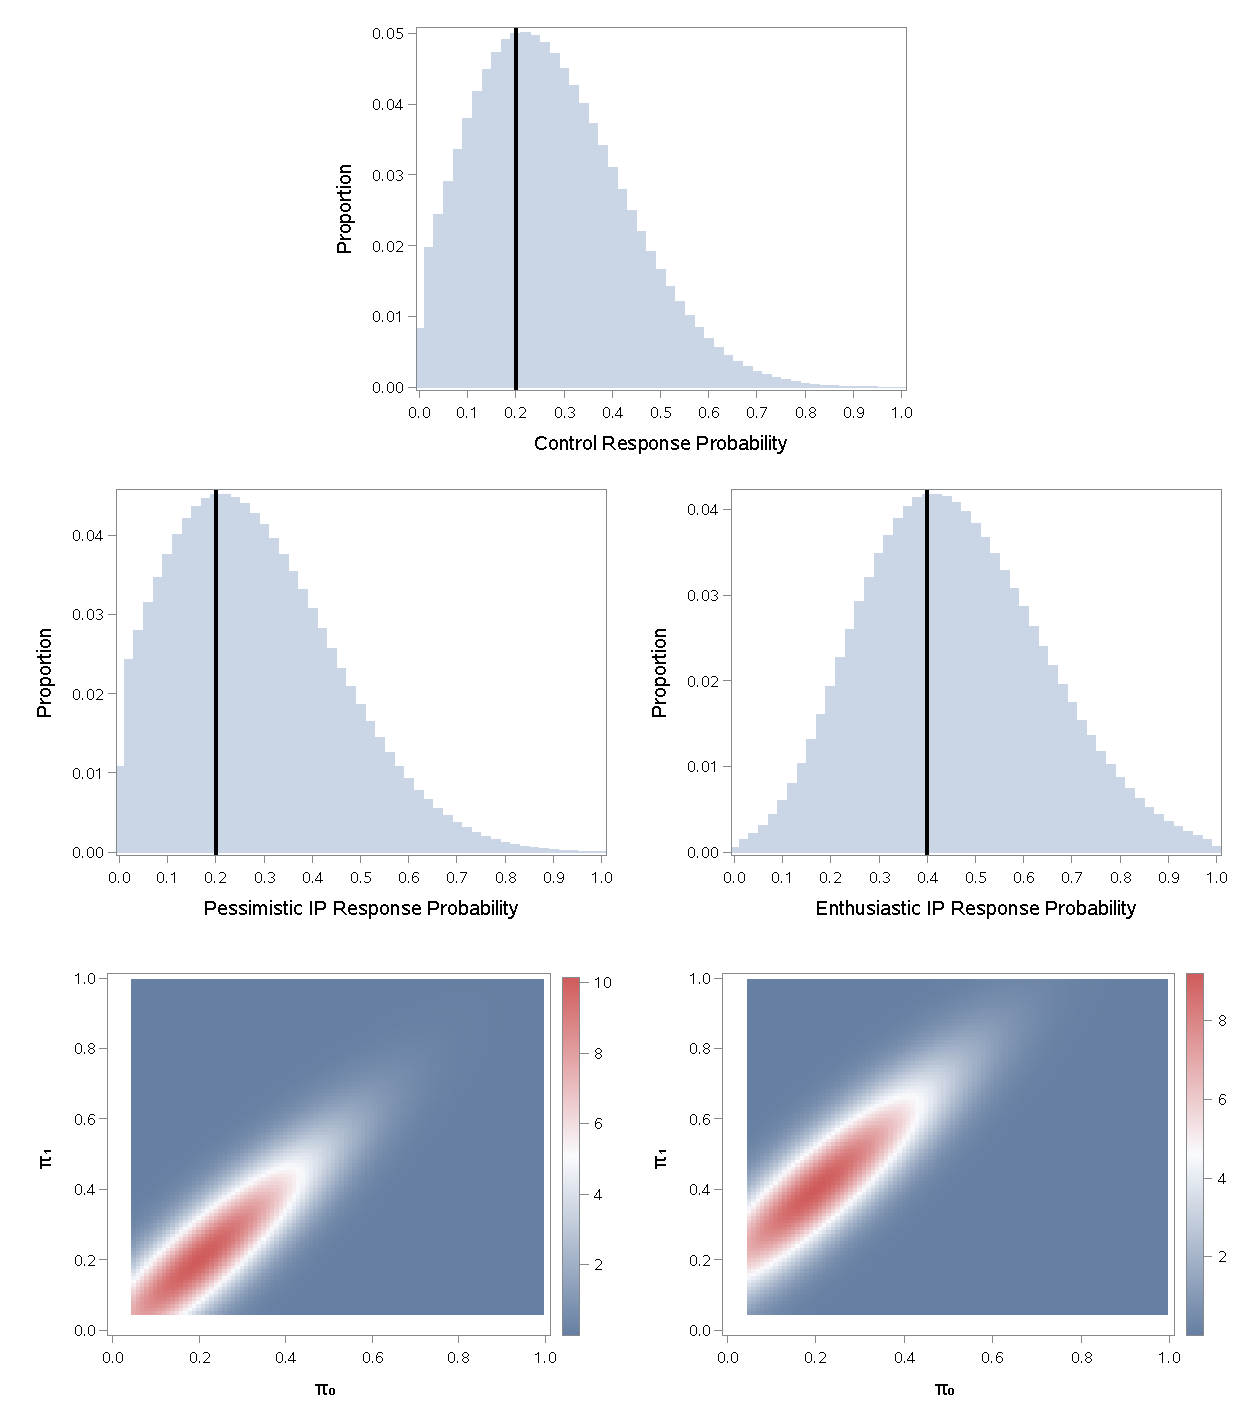
\includegraphics[scale=0.70]{./FIGURES/BINARY-PRIORS.pdf}
%      \caption{Prior for Control Group Response Probability \label{fig:pmp}}
%    \end{figure}
			
	

%\bigskip
\newpage
\begin{center}
{\large\bf SUPPLEMENTARY MATERIAL}
\end{center}


\section{BibTeX}

 \bibliographystyle{agsm}
 \bibliography{./References}		

\end{document}
